\documentclass{article}
\usepackage[utf8]{inputenc}
\usepackage{tikz}
\usepackage{float}
\usepackage{amsmath}
\usepackage[numbers]{natbib}
\usepackage{todonotes}
\usepackage{bm}
\usepackage{setspace}
\usepackage{subcaption}
\usepackage{caption}
\usepackage{textcomp}
\captionsetup{font=footnotesize}
\usepackage[margin=.8in]{geometry}
\usepackage{algorithm}
\usepackage{algpseudocode}
\usepackage{url}
% Thing Dave added these
\usepackage{amssymb}
\usepackage{amsthm}
\newtheorem{theorem}{Theorem}
\usepackage{changes}

 \doublespacing
\title{Analysis of the Elevated Incidence and Case-Fatality Ratio in the Navajo Nation of New Mexico}
\author{Graham Casey Gibson$^{1}$, Luis Valdez$^{2}$}
\date{%
    $^1$Department of Biostatistics and Epidemiology, University of Massachusetts-Amherst, Amherst,
Massachusetts, United States of America\\%
    $^2$Department of Health Promotion and Policy, University of Massachusetts-Amherst, Amherst,
Massachusetts, United States of America\\[2ex]%\\
    \smallskip
    \today
}


\begin{document}

\maketitle
\abstract{

\subsubsection*{Author Summary} 

\section{Introduction}
The Navajo nation has been particularly hit by COVID-19 in terms of both deaths per capita and infections per capita. Recently, the growth rate of cases reached the highest in the nation, with 2304 cases of COVID-19 per 100000 people. In comparison, New York has a rate of 1806  per 100000 people, making the Navajo nation the place with the highest growth rate. 
This is leads to the question of why COVID-19 has been able to spread so easily and cause such damage to the Navajo Nation? This is especially worrying in light of the obvious growth rate factors largely being absent in from the Navajo community. For instance, population density is a known driver of infectious disease spread, yet the Navajo Nation has one of the lowest population densities in the U.S. Second, the mortality rate is almost twice that of the general U.S. population, even though the Navajo Nation is on average younger. To help explain these inconsistencies, we developed the following analysis. 

We first gathered data using the New Mexico Department of Health (NMDOH) health survey dataset. This allows us to compare counties within NM that belong to the Navajo Nation, versus those that do not along key covariates of interest. This study design also helps mitigate geographical confounders, such as humidity and temperature that may impact growth rate of the COVID-19 (although this is an open question). As we can see in Figure \ref{fig:nn},  the Navajo Nation is relatively well clustered in the Northwest corner of the state, and falls within five counties. This allows us to analyze the New Mexico county level growth rates against the NMDOH county level health dataset to gain insight into potential drivers of elevated growth in the Navajo Nation. 

\subsection{Data}


\begin{figure}
\centering
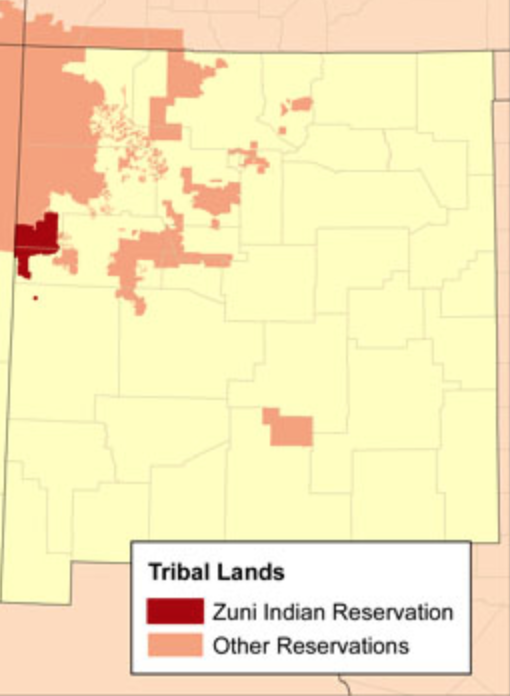
\includegraphics[scale=.75]{navajo_nation_nm}
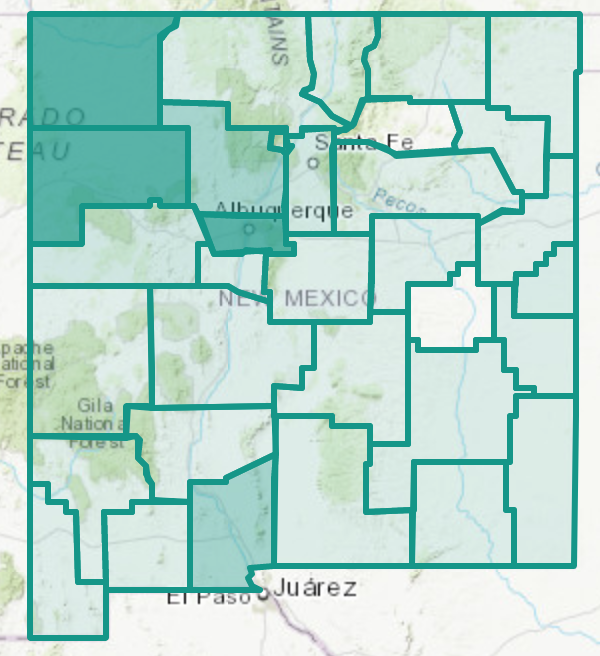
\includegraphics[scale=.75]{nn_covid}
\caption{Left: Navajo Nation Boundaries for New Mexico. Right: COVID-19 cases as of June 17th 2020 according to the New Mexico Department of Health. We can immediately see that the northwest corner of the state has both the most cases (raw count) and is part of the Navajo Nation territory.  } 
\label{fig:nn}

\end{figure}

\begin{figure}
\centering
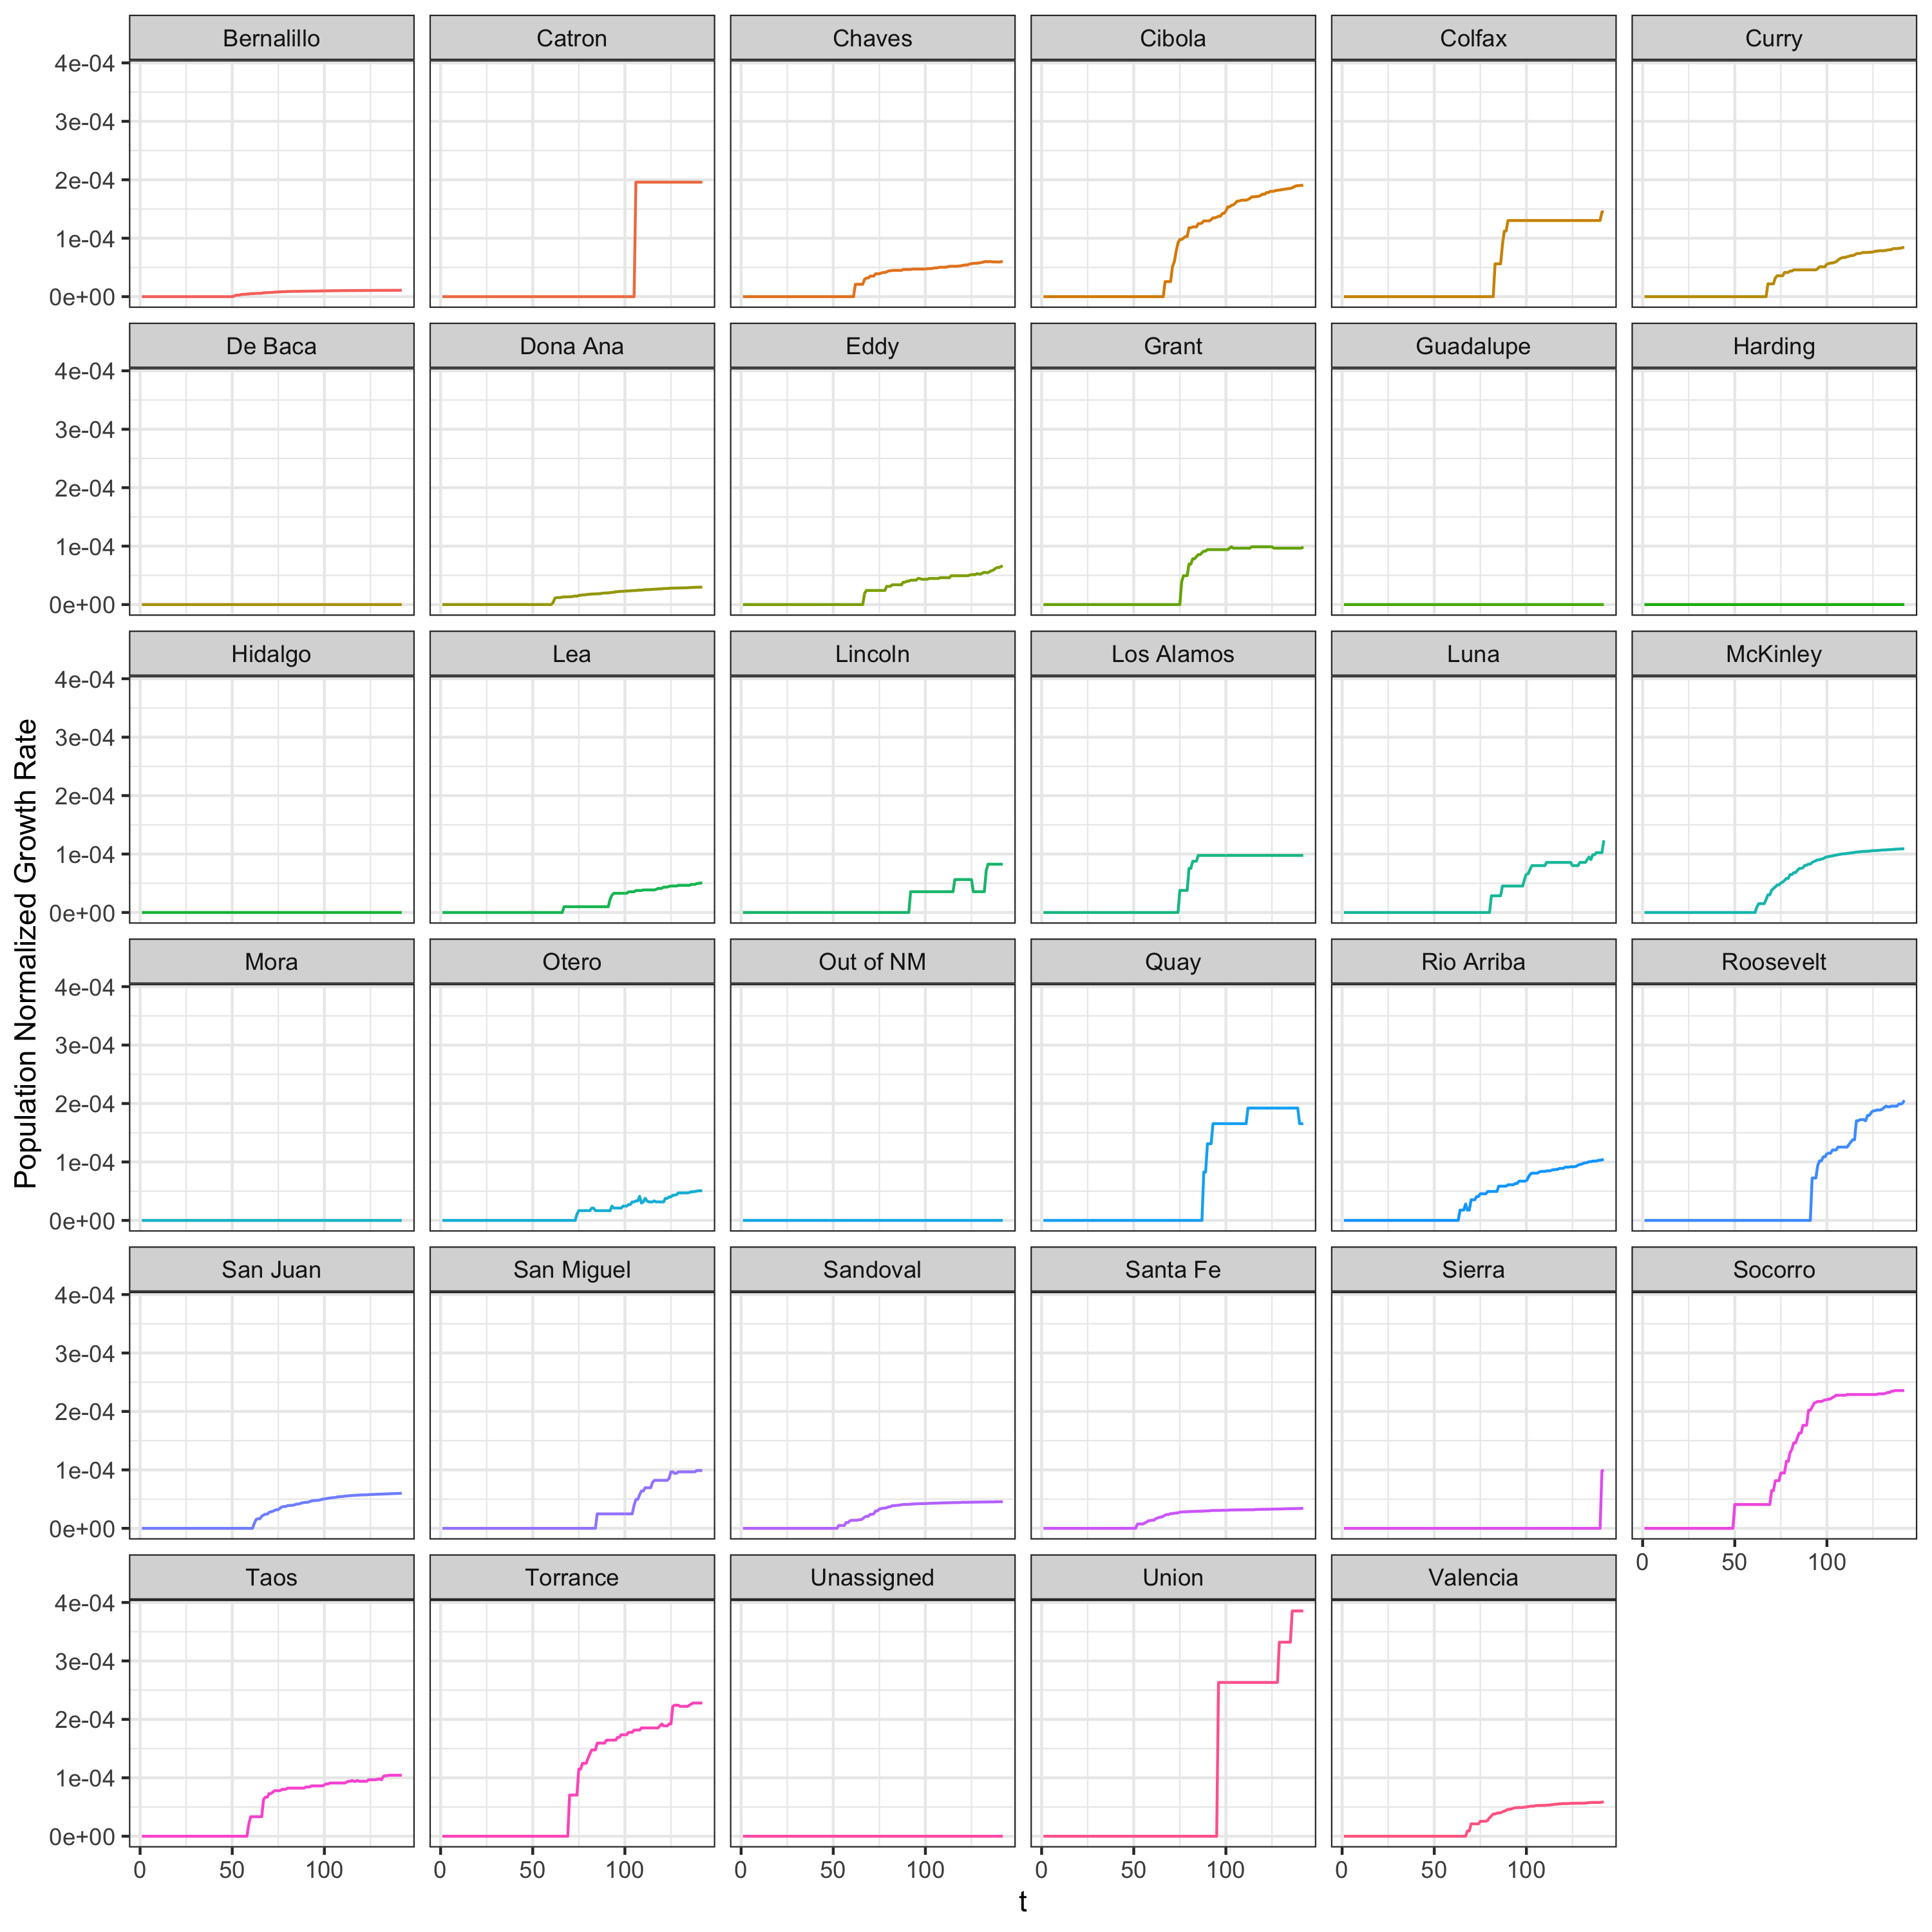
\includegraphics[scale=.15]{log_case_plot.png}
\caption{Population normalized log case counts by county in New Mexico. This is computed by taking the cases over time, dividing by population size and taking the natural logarithm. We can clearly see heterogeneity amongst the growth rates by county.   }
\label{fig:data}
\end{figure}


We first present the growth rates of COVID-19 by county.  As we can see in Figure \ref{fig:data}, the population normalized growth rates are much higher for the two Navajo Nation communities relative to the metro centers of New Mexico. This suggests that something besides population density and age-structure is driving the elevated growth rate. 


In order to examine the effects of covariates on growth rates, we employ the auto-regressive moving average framework, as implemented in the Forecast package in R (cite forecast).  We do this to capture both the temporal correlation between cases and because COVID19 has been demonstrated to follow an exponential growth curve (cite something here), which in log space can be described by a linear model, such as an autoregressive model. 

\begin{equation}
 log(c_t) = \alpha + \phi log(c_{t-1}) + \theta\epsilon_{t-1} + \bm{\gamma} \bm{X} + \epsilon_t
 \end{equation}

where $X$ is the design matrix with columns,

$$\text{columns(X)} = \{\text{Population Density}  \ , \text{Food Insecurity} \ ,  \text{Multigenerational Household} \ , \text{Healthcare Access} \ , \text{Mean Age Distribution}\}$$


where covariates do not change over time. We have omitted intervention covariates since all counties were subject to the same state-wide intervention efforts. There may be heterogeneity across counties in terms of compliance, but we lack data to adjust for this so we remove it from the analysis. 

\subsubsection{Covariate Data}

We now take a closer look at the data used to inform COVID-19 growth rates. As we can see from Figure \ref{fig:covariate_data} top left, the two counties that most closely overlap with the Navajo Nation (McKinley and San Juan) more than 10\% of households qualify as multi-generational. However, for the remainder of the state, counties with populations over 20,000 all have multi-generational household percentages <10\%. However, most of the state is is >5\%. This suggests that there is not a huge discrepancy between the percentage of multi-generational households in the Navajo Nation of NM versus the rest of the state.  

As we can see from Figure \ref{fig:covariate_data} top right, healthcare access was on average lower for counties inside the Navajo Nation of NM versus counties outside. The differences between the urban counties (Bernallilo and Santa Fe) and the Navajo Nation of NM counties is roughly 15\%. \textbf{Need to say more here}

As we can see from Figure \ref{fig:covariate_data} bottom left, food insecurity levels were on average higher for counties inside the Navajo Nation of NM versus counties outside. The differences between the urban counties (Bernallilo and Santa Fe) and the Navajo Nation of NM counties is roughly 10\%. \textbf{Need to say more here}

As we can see from Figure \ref{fig:covariate_data} bottom right, population density is drastically higher in the urban centers than in the Navajo Nation of NM counties.  \textbf{Need to say more here}

\begin{figure}
\centering
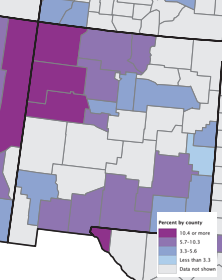
\includegraphics[scale=1.5]{multi-gen-plot}
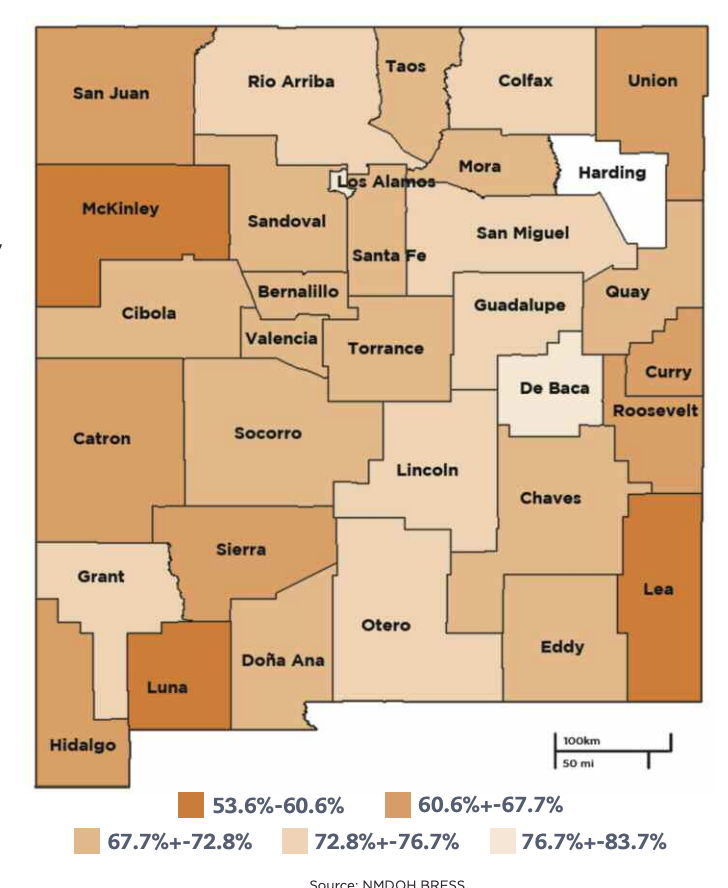
\includegraphics[scale=.5]{access_to_healthcare-plot}
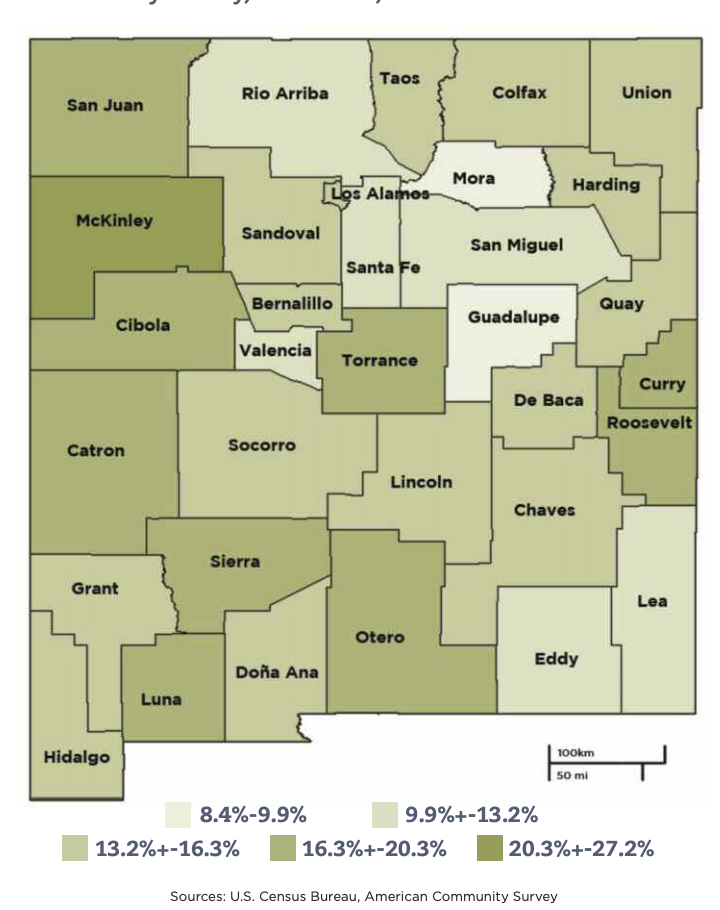
\includegraphics[scale=.5]{food_insecurity-plot}
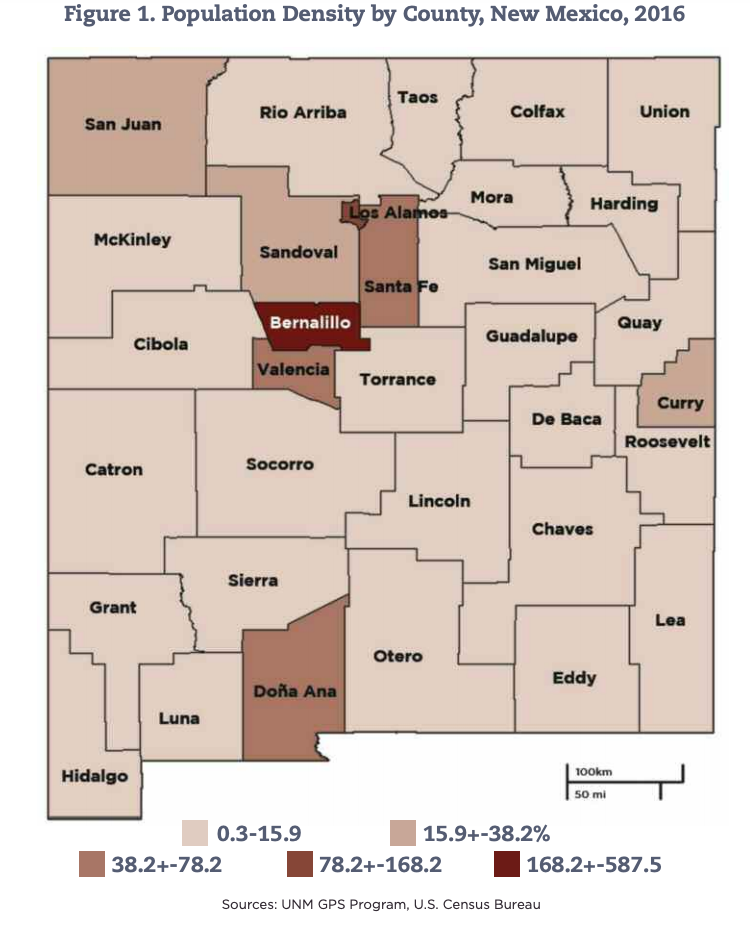
\includegraphics[scale=.5]{pop_density-plot}
\caption{Covariate maps used in the above analysis. \textbf{Top Left} shows the percentage of households that have multiple generations of occupants in the household. \textbf{Top Right} shows the percentage of households in the county that have access to healthcare, as defined by NMDOH. \textbf{Bottom Left} shows the percentage of households in the county facing some level of food insecurity, as defined by NMDOH. \textbf{Bottom Right} shows the population density of each county, as defined by NMDOH.  }
\label{fig:covariate_data}
\end{figure}




\subsection{Methods}

We use the covariate data described above 


\subsection{Results}




\subsection{Discussion}






\newpage
\bibliographystyle{unsrt}
\bibliography{bib}











\end{document}